\begin{document}

\frame{\titlepage}
\note{Introductions!}

\frame{
    \frametitle{Motivation}

    Collagen-based artificial vessels have applications in two key surgical contexts.

    \begin{columns}[t, onlytextwidth]
        \column{0.48\textwidth}
        \begin{block}{Haemodialysis}
            \begin{itemize}
                \item Blood is removed, processed in a dialyser, then replaced
                \item Requires reliable vascular access at high flow rates
                \item Natural fistulas are difficult to achieve in elderly patients
            \end{itemize}
        \end{block}

        \column{0.48\textwidth}
        \begin{block}{Bypass surgery}
            \begin{itemize}
                \item New routes are created for blood flow
                \item Artificial grafts offer standardisation and greater availability
            \end{itemize}
        \end{block}
    \end{columns}
}
\note{
    \textbf{Tahmid}
    \begin{itemize}
        \item Discuss why haemodialysis first over bypass surgery (non life-threatening medical device, easily classification and entry into the market, and shorter duration in the body)
    \end{itemize}
}

\frame{
    \frametitle{Arteriovenous fistula}
    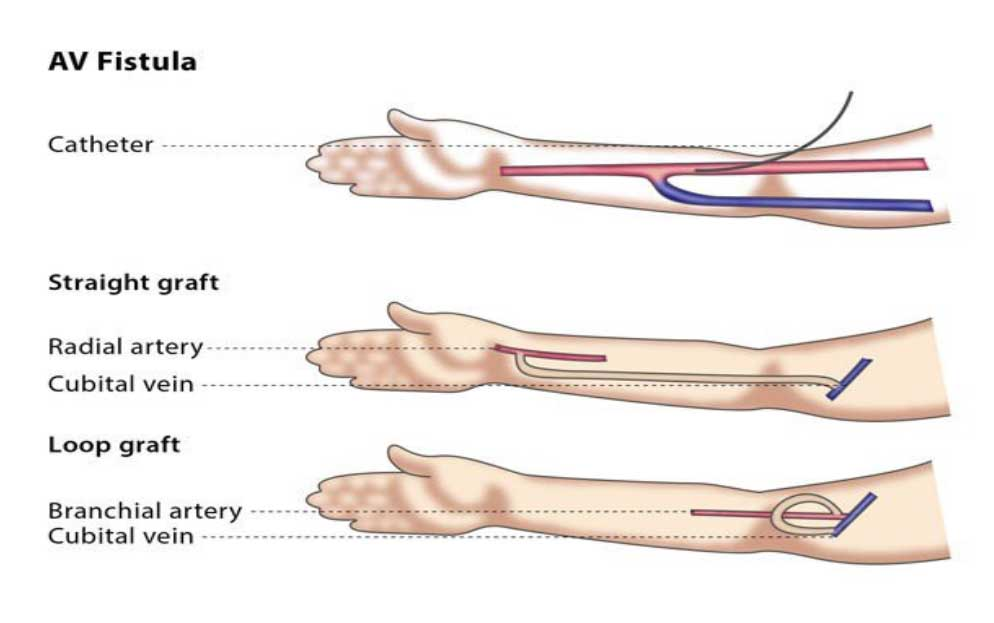
\includegraphics[width=\textwidth]{images/av_fistula_graft.jpg}
}
\note{
    \textbf{Tahmid}
    \begin{itemize}
        \item Describe natural vascular changes with aging
        \item Describe iatrogenic vascular changes (e.g. repeated use of superficial veins)
        \item Prolonged time to maturation in the elderly (normally 6--12 weeks)
    \end{itemize}
}


\frame{
    \frametitle{Existing laboratory bench}

    \centering
    \resizebox{\textwidth}{!}{%
        \begin{tikzpicture}[
                box/.style={draw, rounded corners=2pt, minimum height=12mm, minimum width=28mm, align=center, inner sep=5pt, font=\large},
                sensor/.style={box, fill=gray!10},
                logger/.style={box, fill=blue!10},
                arr/.style={-Stealth, thick},
                sig/.style={-Stealth, dashed, thick},
            ]

            % Main circuit:
            \node[box] (res)  at (0,   0) {Reservoir};
            \node[box] (pump) at (3.8, 0) {Peristaltic\\pump};
            \node[box] (rt1)  at (7.6, 0) {Resistance\\tubing};
            \node[box] (ves)  at (14.1, 0) {Test\\vessel};
            \node[box] (rt2)  at (20.6, 0) {Downstream\\resistance};

            % Flow arrows with the return loop going over the top:
            \draw[arr] (res) -- (pump);
            \draw[arr] (pump) -- (rt1);
            \draw[arr] (rt1) -- (ves);
            \draw[arr] (ves) -- (rt2);
            \draw[arr] (rt2.north) -- ++(0,0.8) -- ($(res.north)+(0,0.8)$) -- (res.north);

            % Pressure sensor taps with sensors below the main flow and arrows pointing toward flow line:
            \coordinate (tap1) at ($(rt1.east)!0.5!(ves.west)$);
            \coordinate (tap2) at ($(ves.east)!0.5!(rt2.west)$);
            \node[sensor] (p1) at ($(tap1)+(0,-1.8)$) {$P_1$};
            \node[sensor] (p2) at ($(tap2)+(0,-1.8)$) {$P_2$};
            \draw[arr] (p1.north) -- (tap1);
            \draw[arr] (p2.north) -- (tap2);

            % Optical micrometer below the vessel, arrow pointing toward vessel:
            \node[sensor] (mic) at ($(ves)+(0,-1.8)$) {Optical\\micrometer};
            \draw[arr] (mic.north) -- (ves.south);

            % Data logger below sensors:
            \node[logger] (dl) at ($(ves)+(0,-3.8)$) {Data\\logger};

            % Signal lines:
            \draw[sig] (p1.south)  |- (dl.west);
            \draw[sig] (p2.south)  |- (dl.east);
            \draw[sig] (mic.south) -- (dl.north);
        \end{tikzpicture}
    }

    \begin{alertblock}{Limitations}
        \begin{itemize}
            \item Excess tubing creates a cluttered workspace
            \item Achieving \SI{300}{\milli\liter\per\minute} requires more than \SI{250}{rpm} $\gg$ resting cardiac frequency range, \SIrange{60}{120}{bpm}
        \end{itemize}
    \end{alertblock}
}
\note{
    \scriptsize
    \textbf{Luca}
    \begin{itemize}
        \item Went to see the current 4th year project setup
              \begin{itemize}
                  \scriptsize
                  \item Consists of a peristaltic pump where flow rate can be modified
                  \item Compliance tubing to smooth out pulses from the pump
                  \item Enters test section where the vessel diameter is tracked using an optical micrometer, and the pressure profile is detected using a differential pressure sensor
                  \item Downstream resistance tubing provides a back pressure that changes the mean pressure of the profile
              \end{itemize}
        \item Main problem areas:
              \begin{itemize}
                  \scriptsize
                  \item Large offset from atmospheric pressure means pressure resolution isn't ideal
                  \item Tubing creates a cluttered test area
                  \item Cannot model flow rates of 300mL/min as creates non-realistic heart rates of 350bpm
              \end{itemize}
    \end{itemize}
}

\frame{
    \frametitle{Design brief}

    \begin{columns}[t, onlytextwidth]
        \column{0.48\textwidth}
        \begin{block}{Requirements}
            \begin{itemize}
                \item Continuous flow for \SI{90}{\minute}
                \item Mean perfusion pressure \SIrange{80}{120}{mmHg}
                \item Compatible with \SI{6}{\milli\meter} OD tubing
                \item Closed-loop control via pressure sensing
                \item Non-destructive to RBCs and endothelial layer
            \end{itemize}
        \end{block}

        \column{0.48\textwidth}
        \begin{block}{Desiderata}
            \begin{itemize}
                \item Physiologically realistic pulsatile pressure profile
                \item Multiple pumps in parallel
                \item Selectable pre-programmed flow profiles
                \item Burst pressure ramp protocol
                \item Peak flow rate \SI{300}{\milli\liter\per\minute}
            \end{itemize}
        \end{block}
    \end{columns}
}
\note{
    \scriptsize
    \textbf{Luca}
    \begin{itemize}
        \item After the meeting with Dr Markaki, developed design brief for our pump
        \item Split into a list of desirable and essential features
        \item Key performance indicators are:
              \begin{itemize}
                  \scriptsize
                  \item 90 min runtime
                  \item Mean pressure between 80--120mmHg
                  \item Pressure adjustment via closed loop control
                  \item Non-destructive to RBC's
              \end{itemize}
        \item The desirable functions are:
              \begin{itemize}
                  \scriptsize
                  \item Optimise the pressure profile so that it is physiologically realistic
                  \item Design a system so multiple pumps can be used in parallel
                  \item Have pre-programmed profiles for different vessels and ages/conditions
                  \item Test the burst pressure of the grafts by using a pressure ramp
                  \item Achieve a peak flow rate of 300ml/min
              \end{itemize}
    \end{itemize}
}

\frame{
    \frametitle{Initial design: syringe pump}

    \begin{itemize}
        \item 2 syringes for continuous flow
        \item Valves prevent backflow
        \item Pinch valves/motor variation to create non-standard waveform
        \item Pressure sensors for a feedback loop
    \end{itemize}
}
\note{\textbf{Lucy}}

\frame{
    \frametitle{Initial design: syringe pump}
    \centering
    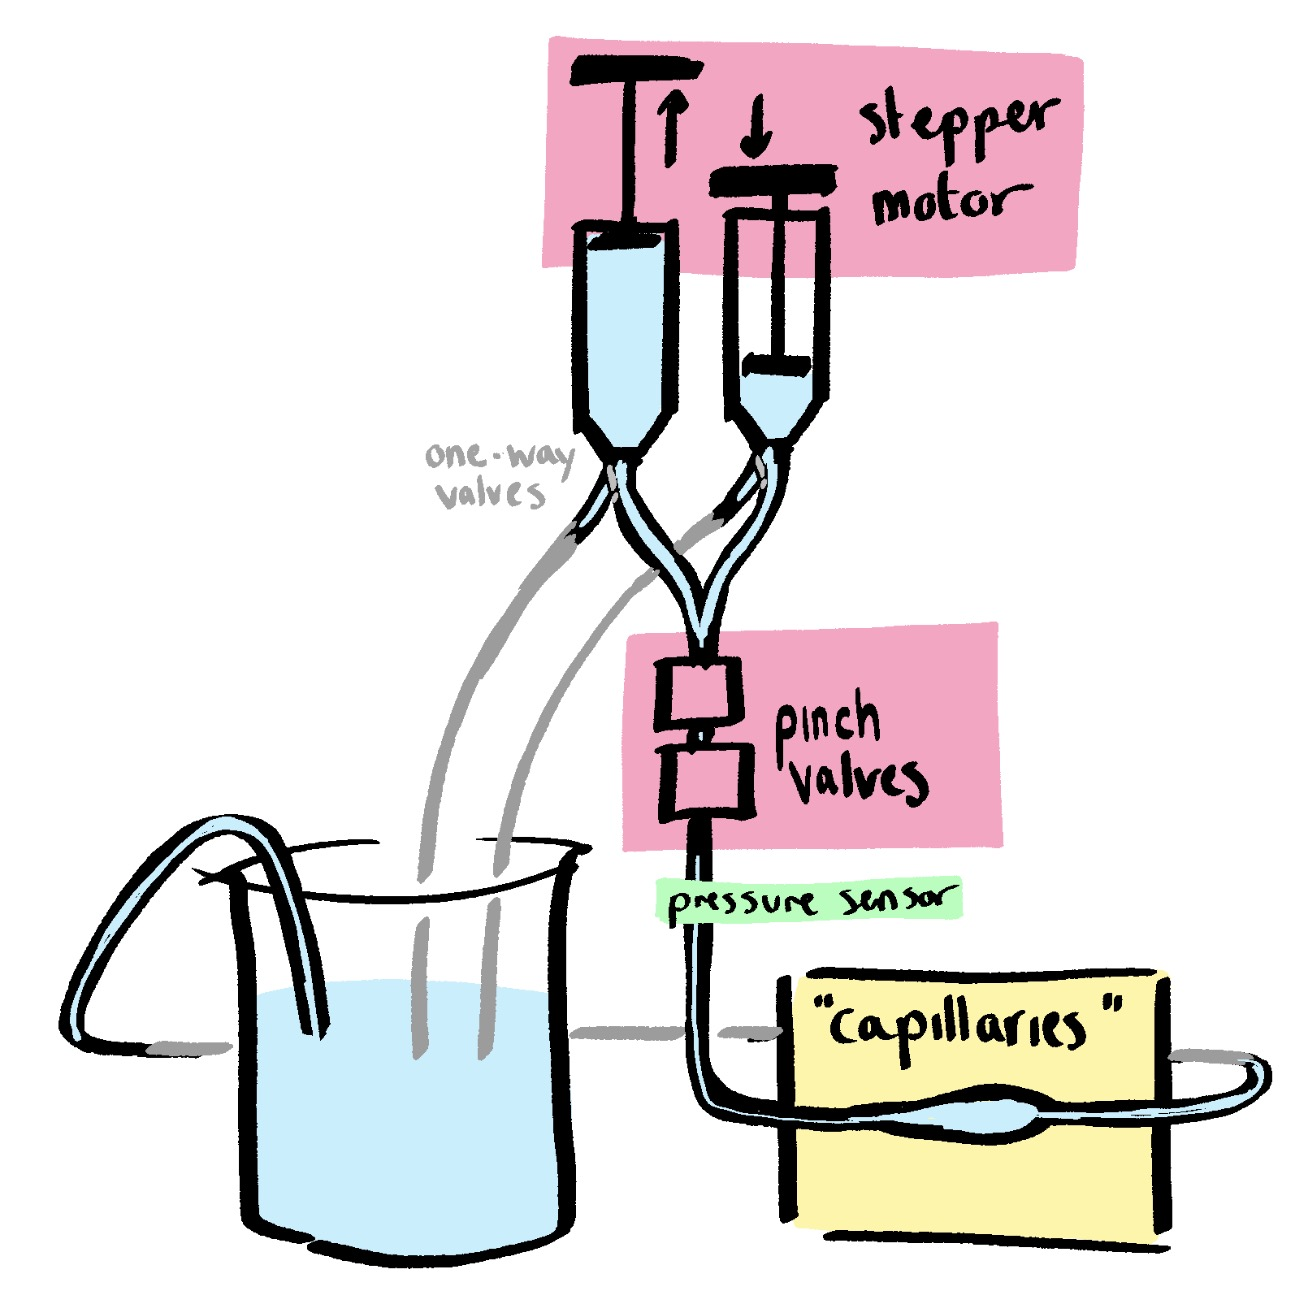
\includegraphics[width=0.8\textwidth]{images/design.jpg}
}
\note{\textbf{Lucy}}

\frame{
    \frametitle{Project resources}
    \centering

    \small
    \begin{tabular}{lll}
        \hline
        \textbf{item}               & \textbf{qty.} & \textbf{unit cost (£)} \\
        \hline
        microcontroller             & 1             & 20                     \\
        motor controller board      & 1             & 20                     \\
        lead screw \& stepper motor & 2             & 15                     \\
        pressure sensors            & 2             & 10                     \\
        one-way valves              & 4             & 2                      \\
        3/2 valves                  & 2             & 10                     \\
        pinch valves                & 2             & 20                     \\
        syringes                    & 2+            & 1                      \\
        tubing                      & ---           & 10                     \\
        simple alphanumeric display & 1             & 10                     \\
        T-type connectors           & 2             & 1                      \\
        \hline
        \multicolumn{3}{l}{\textit{Departmental}}                            \\
        \hline
        3D printer                  & ---           & ---                    \\
        housing material            & ---           & ---                    \\
        \hline
        \textbf{total}              &               & $\sim$\textbf{150}     \\
        \hline
    \end{tabular}
}
\note{
    \scriptsize
    \textbf{Lonnie}
    \begin{itemize}
        \tiny
        \item Microcontroller --- controls the pressure profile and monitors flow rate throughout the system
        \item Power board --- converts 240V mains supply down to 5V for use by the electronics
        \item Lead screw \& stepper motor --- pushes and retracts the syringe accurately to displace precise fluid volumes
        \item Pressure sensors --- measure the pressure profile within the test section to close the feedback loop
        \item One-way valves --- prevent backflow from the syringe into the test section during retraction
        \item 3/2 valves --- provide an alternative to one-way valves with more flexible flow path switching
        \item Pinch valves --- create a controlled pressure drop to set the downstream resistance
        \item Syringes --- provide a consistent and controllable flow rate into the circuit
        \item Alphanumeric display --- shows real-time flow rate and minimum, peak, and average pressure readings to the user
        \item T-type connectors --- allow fluid to branch into the pressure sensors without disrupting the main flow path
    \end{itemize}
}


\frame{
    \frametitle{Final product cost}
    \centering

    \small
    \begin{tabular}{lll}
        \hline
        \textbf{item}               & \textbf{qty.} & \textbf{unit cost (£)} \\
        \hline
        microcontroller             & 1             & 5--20                  \\
        motor controller board      & 1             & 10--20                 \\
        lead screw \& stepper motor & 2             & 15                     \\
        pressure sensors            & 2             & 3--10                  \\
        valves                      & 2--6          & 2                      \\
        syringes                    & 2             & 1                      \\
        tubing                      & ---           & ---                    \\
        \hline
        \textbf{total}              &               & \textbf{50--100}       \\
        \hline
        commerical syringe pumps    &               & 250--3000              \\
        \hline
    \end{tabular}
}
\note{
    \textbf{Lonnie}
}

\frame{
    \frametitle{Timeline}
    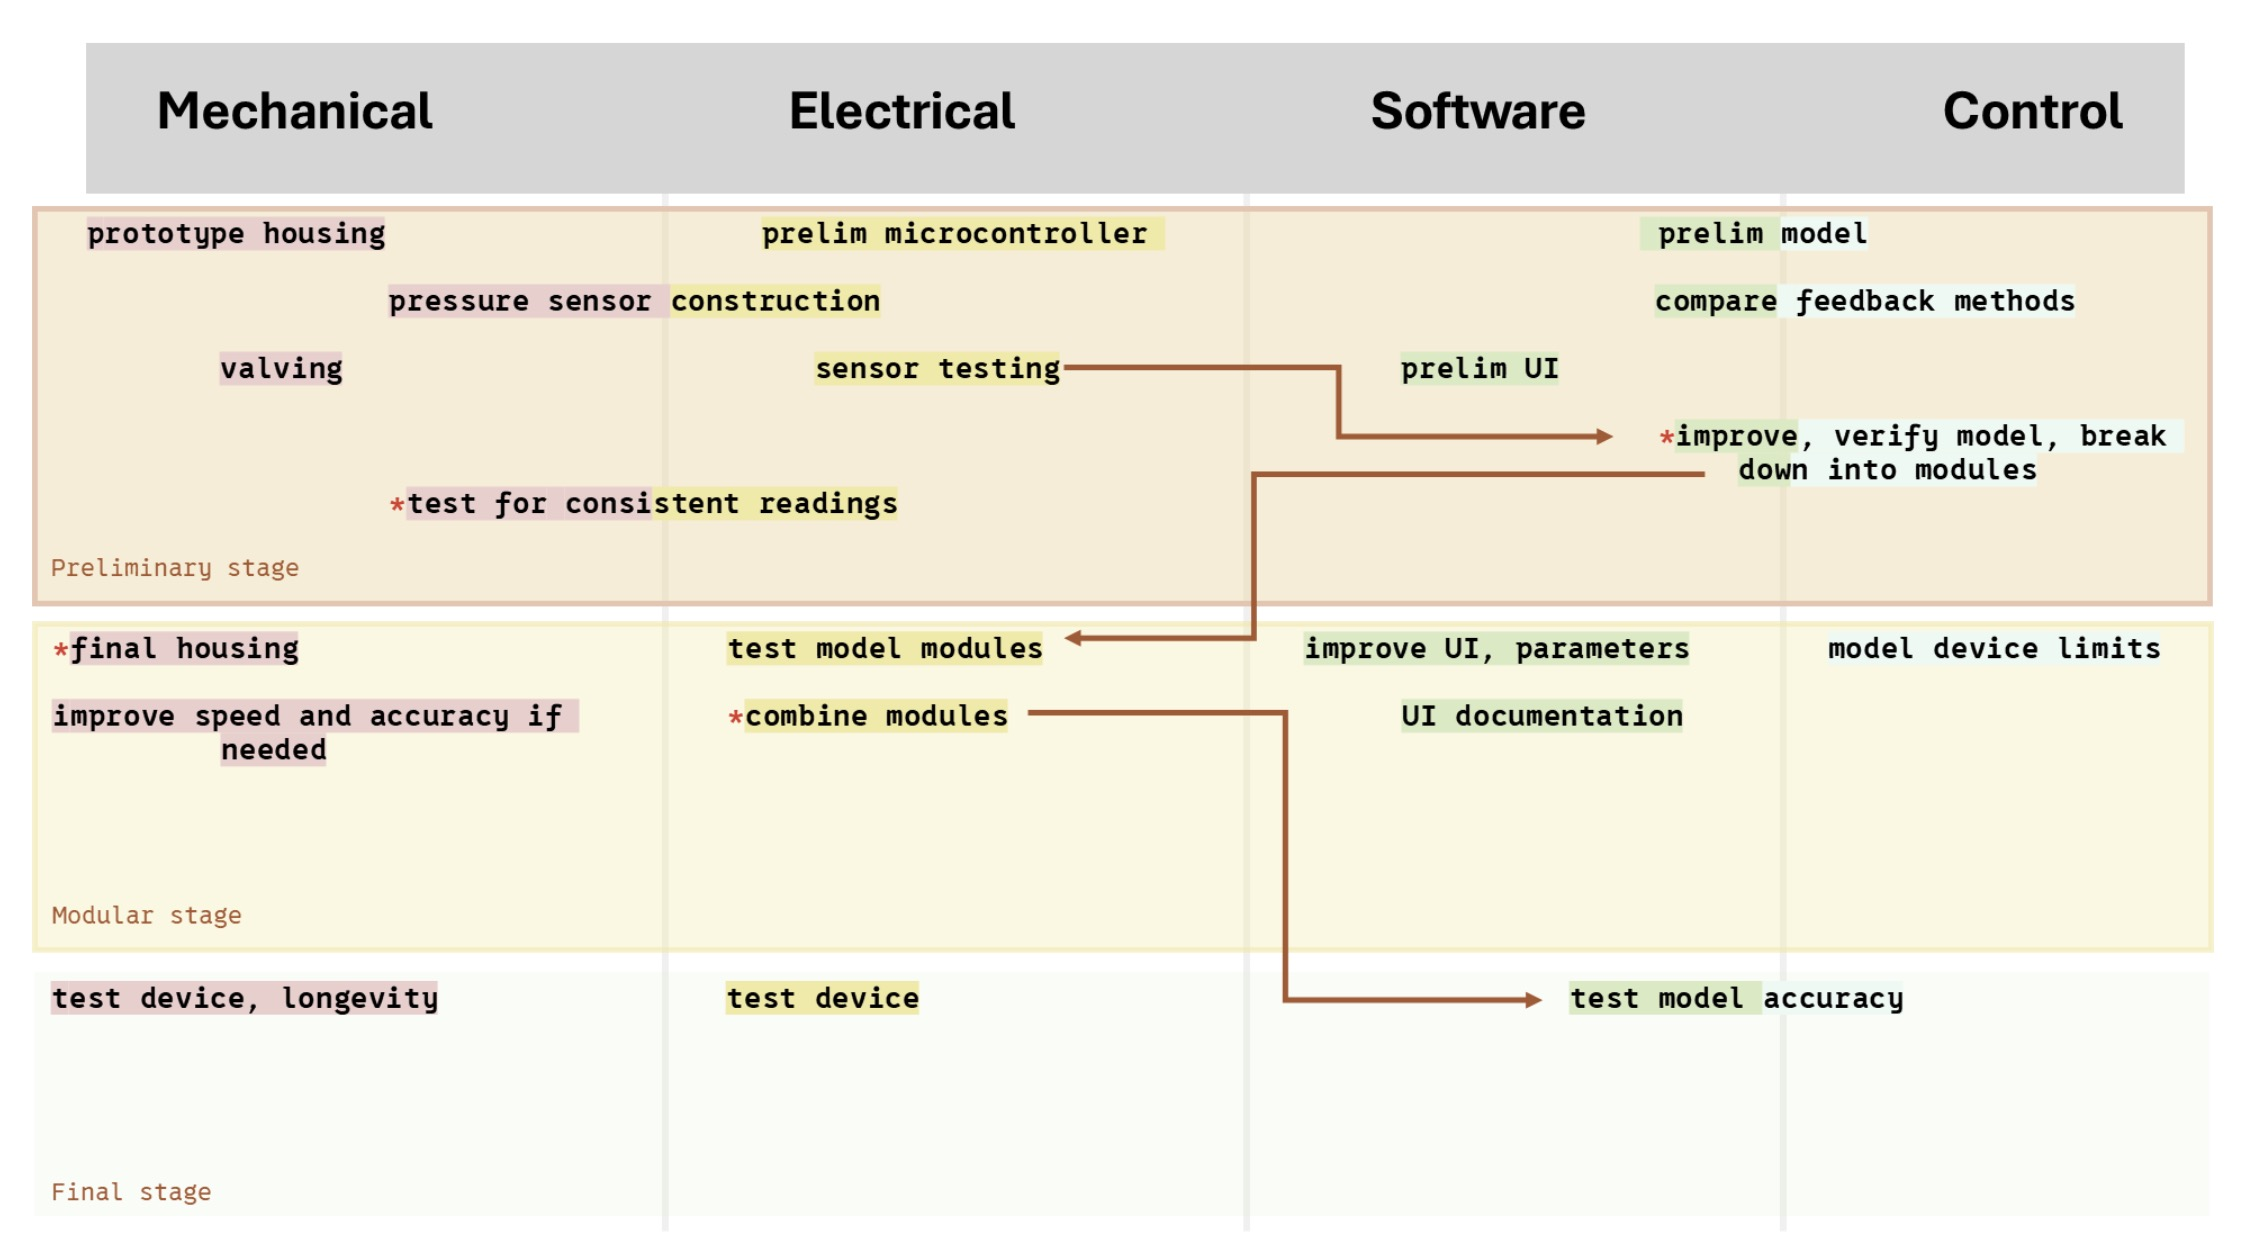
\includegraphics[width=\textwidth]{images/gantt.jpg}
}
\note{
    \textbf{Lonnie}
}

\frame{
    \frametitle{Mechanical}

    \begin{itemize}
        \item Design housing for motors, syringes, and reservoir
        \item Design and assemble connections for pressure sensors
        \item Design and assemble valve junctions
        \item Data collection for control system parameter tuning
        \item Ensure final product is easy to 3D print and assemble, and that multiple pumps can be made and run at once
    \end{itemize}

    \centering

    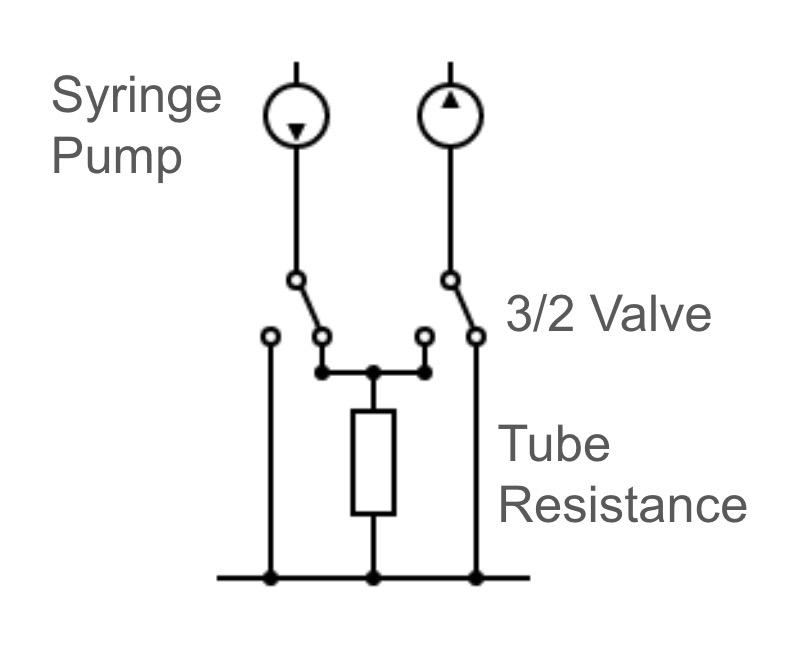
\includegraphics[width=0.4\textwidth]{images/circuit.jpg}
}
\note{
    \textbf{Lucy}
}



\frame{
    \frametitle{Mechanical: pressure sensing specifications}

    \centering\small
    \begin{tabular}{llp{0.42\textwidth}}
        \hline
        \textbf{parameter} & \textbf{value}           & \textbf{rationale}                                                                     \\
        \hline
        Operating range    & \SIrange{80}{120}{mmHg}  & Physiological perfusion target at rest                                                 \\
        Full range         & \SIrange{150}{500}{mmHg} & Burst testing and safety margins                                                       \\
        Sensor type        & Gauge                    & Eliminates \SI{760}{mmHg} atmospheric offset to avoid sacrificing sensor dynamic range \\
        Minimum bandwidth  & \SI{100}{\hertz}         & Nyquist for estimated \SI{50}{\hertz} control loop sampling rate                       \\
        \hline
    \end{tabular}
}
\note{
    \textbf{India}

    \begin{itemize}
        \item Pressure is the primary output variable, the physiological signal being replicated
        \item Closed-loop control drives the pump to track a target pressure waveform
        \item Mean perfusion pressure must be maintained in a range, e.g. \SIrange{80}{120}{mmHg} at rest
        \item The heart beats at ${\sim}\SI{1}{\hertz}$, but fast transients in the waveform must be faithfully tracked
    \end{itemize}
}

\frame{
    \frametitle{Mechanical: valves}

    \begin{itemize}
        \item 2 one-way valves at syringe exit with the same cracking pressure mechanism as in the heart
        \item Optional 3/2 valve setup for more control
    \end{itemize}

    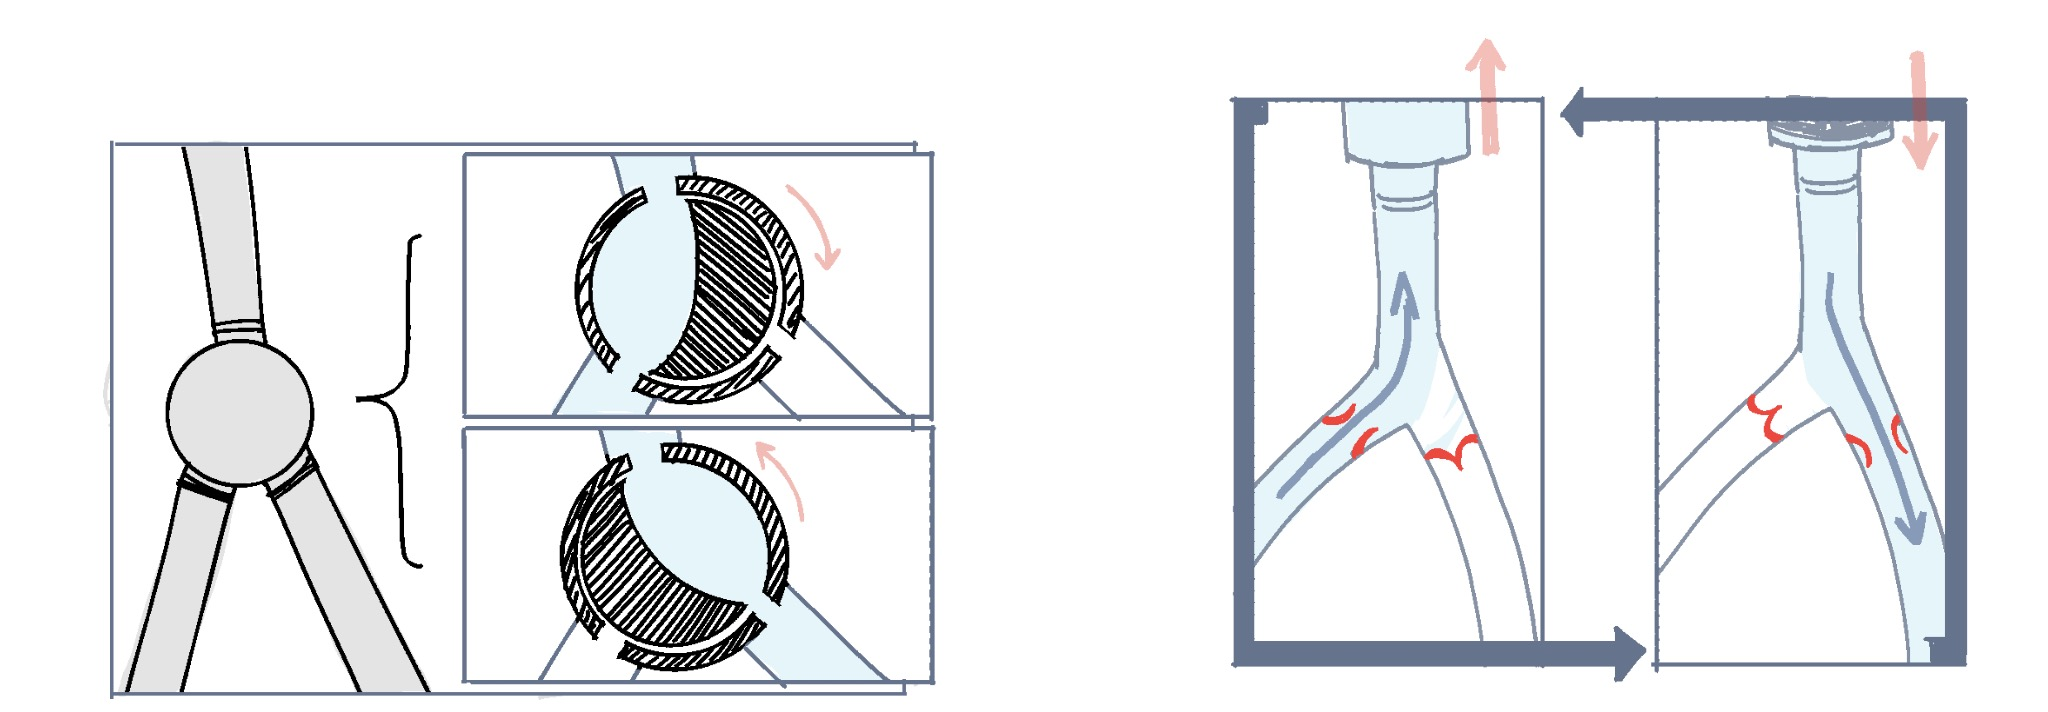
\includegraphics[width=\textwidth]{images/valves.jpg}
}
\note{
    \textbf{Lucy}
}

\frame{
    \frametitle{Mechanical: motors}

    \begin{block}{Stepper motor}
        \begin{itemize}
            \item Precise position control
            \item Fast, inexpensive speed changes
            \item \SI{200}{steps\per rev}, \SI{0.1}{\newton\meter} hold torque
        \end{itemize}
    \end{block}

    \begin{block}{Key calculations}
        \small
        \[
            n = \frac{60Q}{AL} \approx \SI{37.5}{rpm} \qquad
            T = \frac{FL}{2\pi\eta} \approx \SI{6.8}{\milli\newton\meter}
        \]

        \small N.B. $n$: motor speed; $Q$: flow rate; $A$: syringe area; $L=\SI{8}{\milli\meter}$: lead screw pitch; $T$: torque; $F$: axial force; $\eta$: efficiency
    \end{block}
}
\note{
    \textbf{Luca}
}

\frame{
    \frametitle{Mechanical: waveform}

    \begin{columns}[t,onlytextwidth]
        \column{0.48\textwidth}
        \vspace{0pt}

        \begin{block}{Simpler}
            \begin{itemize}
                \item Stepper motor modulates syringe push rate directly
                \item Only 1 pressure sensor required
            \end{itemize}
        \end{block}

        \column{0.48\textwidth}
        \vspace{0pt}
        \begin{block}{More control}
            \begin{itemize}
                \item Pinch valves added downstream of test section
                \item AC pressure component superimposed on DC syringe output
                \item 2 pressure sensors required
            \end{itemize}
        \end{block}

    \end{columns}
    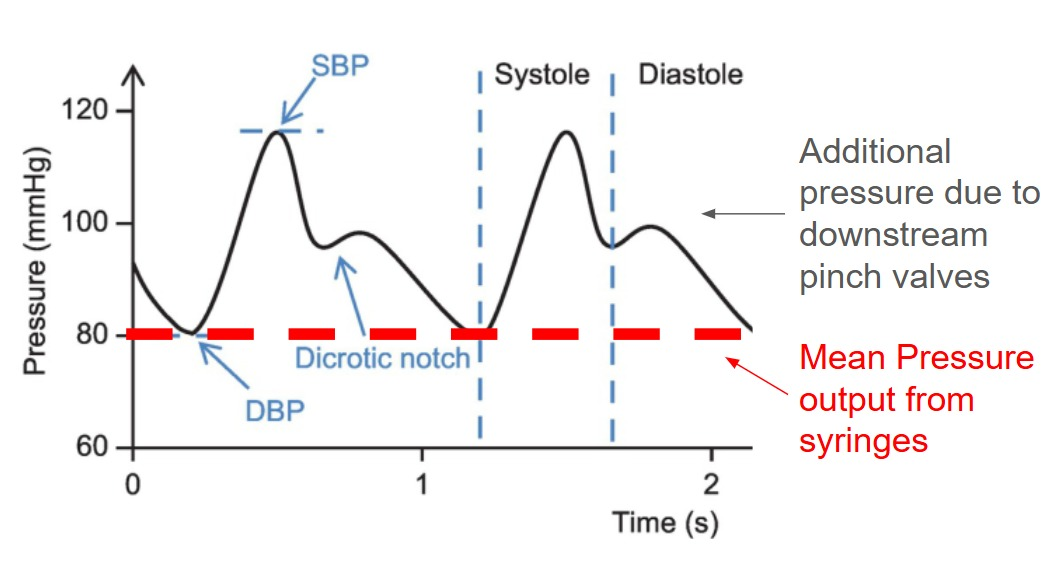
\includegraphics[width=0.6\linewidth,keepaspectratio]{images/lucy_pressure_profile.jpeg}
}
\note{
    \textbf{Luca}
}

\frame{
    \frametitle{Electrical}

    \begin{block}{Preliminary}
        \begin{itemize}
            \item Familiarise with microcontroller
            \item Connect and test sensors
            \item Compare sensor data with control team
        \end{itemize}
    \end{block}

    \begin{block}{Modular}
        \begin{itemize}
            \item Convert model to microcontroller
            \item Combine modules into larger subsystems
            \item Support mechanical team with soldering/other electronic tasks
        \end{itemize}
    \end{block}

    \begin{block}{Final}
        \begin{itemize}
            \item Fix errors using model with control team
            \item Extensive testing
            \item Select cheapest viable microcontroller given features used
        \end{itemize}
    \end{block}
}
\note{
    \textbf{Lonnie}
}

\frame{
    \frametitle{Software}

    \begin{itemize}
        \item Well-documented GUI and CLI (scripting)
        \item Real-time visualisations and plots
        \item Cross-platform
        \item Rich data logging with convenient export formats
    \end{itemize}
}
\note{
    \textbf{Tahmid}
}

\frame{
    \frametitle{Variation of pressure profile with distance}
    \centering
    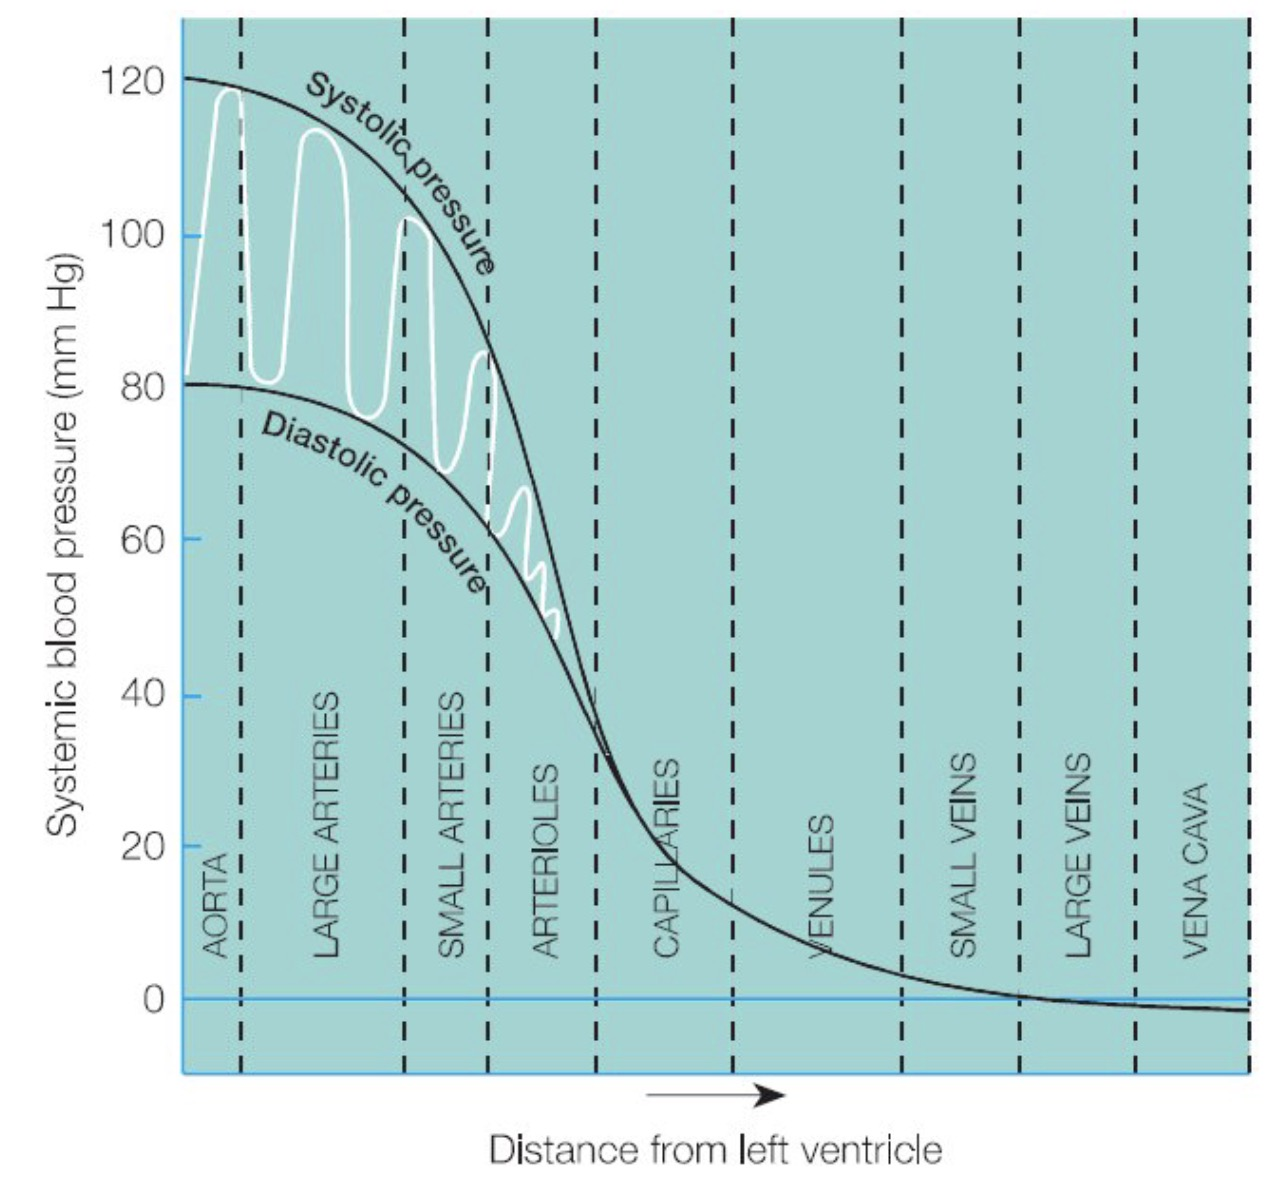
\includegraphics[width=0.7\textwidth]{images/pressure_distance.jpg}
}

\frame{
    \frametitle{Software: profile configuration}

    \begin{itemize}
        \item Customise the target pressure profile via:
              \begin{itemize}
                  \item Physiological parameters (heart rate, systolic/diastolic pressures)
                  \item Demographics (age, sex)
                  \item Activity level (rest vs. exercise)
                  \item Vessel type (artery, capillary, vein)
              \end{itemize}
        \item Set operation schedules
              \begin{itemize}
                  \item e.g.\ ramp pressure to test vessel integrity over time
              \end{itemize}
    \end{itemize}
}
\note{
    \textbf{Tahmid/India}
}

\frame{
    \frametitle{Software: monitoring \& exporting}

    \begin{itemize}
        \item Live pressure trace at the test start point
              \begin{itemize}
                  \item Cumulative error (especially during syringe transition)
                  \item System uptime
              \end{itemize}
        \item Automatic flagging of extreme pressure values
              \begin{itemize}
                  \item Sudden drop $\to$ vessel rupture
                  \item Sudden rise $\to$ blockage or clotting
              \end{itemize}
        \item Export data traces as CSV
    \end{itemize}
}
\note{
    \textbf{Tahmid}
}

\frame{
    \frametitle{Software: modelling the pressure profile}

    \begin{itemize}
        \item Windkessel model to find the mean pressure for a specific vessel
        \item The Womersley number can be used characterise the vessel (inertia dominated, as in large arteries, or viscosity dominated as in capillaries)
        \item Carry out Fourier analysis on parameter-sensitive cardiac waveforms found in literature \cite{malindzakFourierAnalysisCardiovascular1970}
              \begin{equation*}
                  P(t) = P_{\text{mean}} + \sum_{n=1}^{N} A_n \sin(n \omega t + \phi_n)
              \end{equation*}
              Set $\omega$ from heart rate, $P_\text{mean}$ from the Windkessel model and fit $\{A_n\}$ and $\{\phi_n\}$ from literature
    \end{itemize}
}
\note{
    \textbf{Tahmid}
}

\frame{
    \frametitle{Pressure profile}
    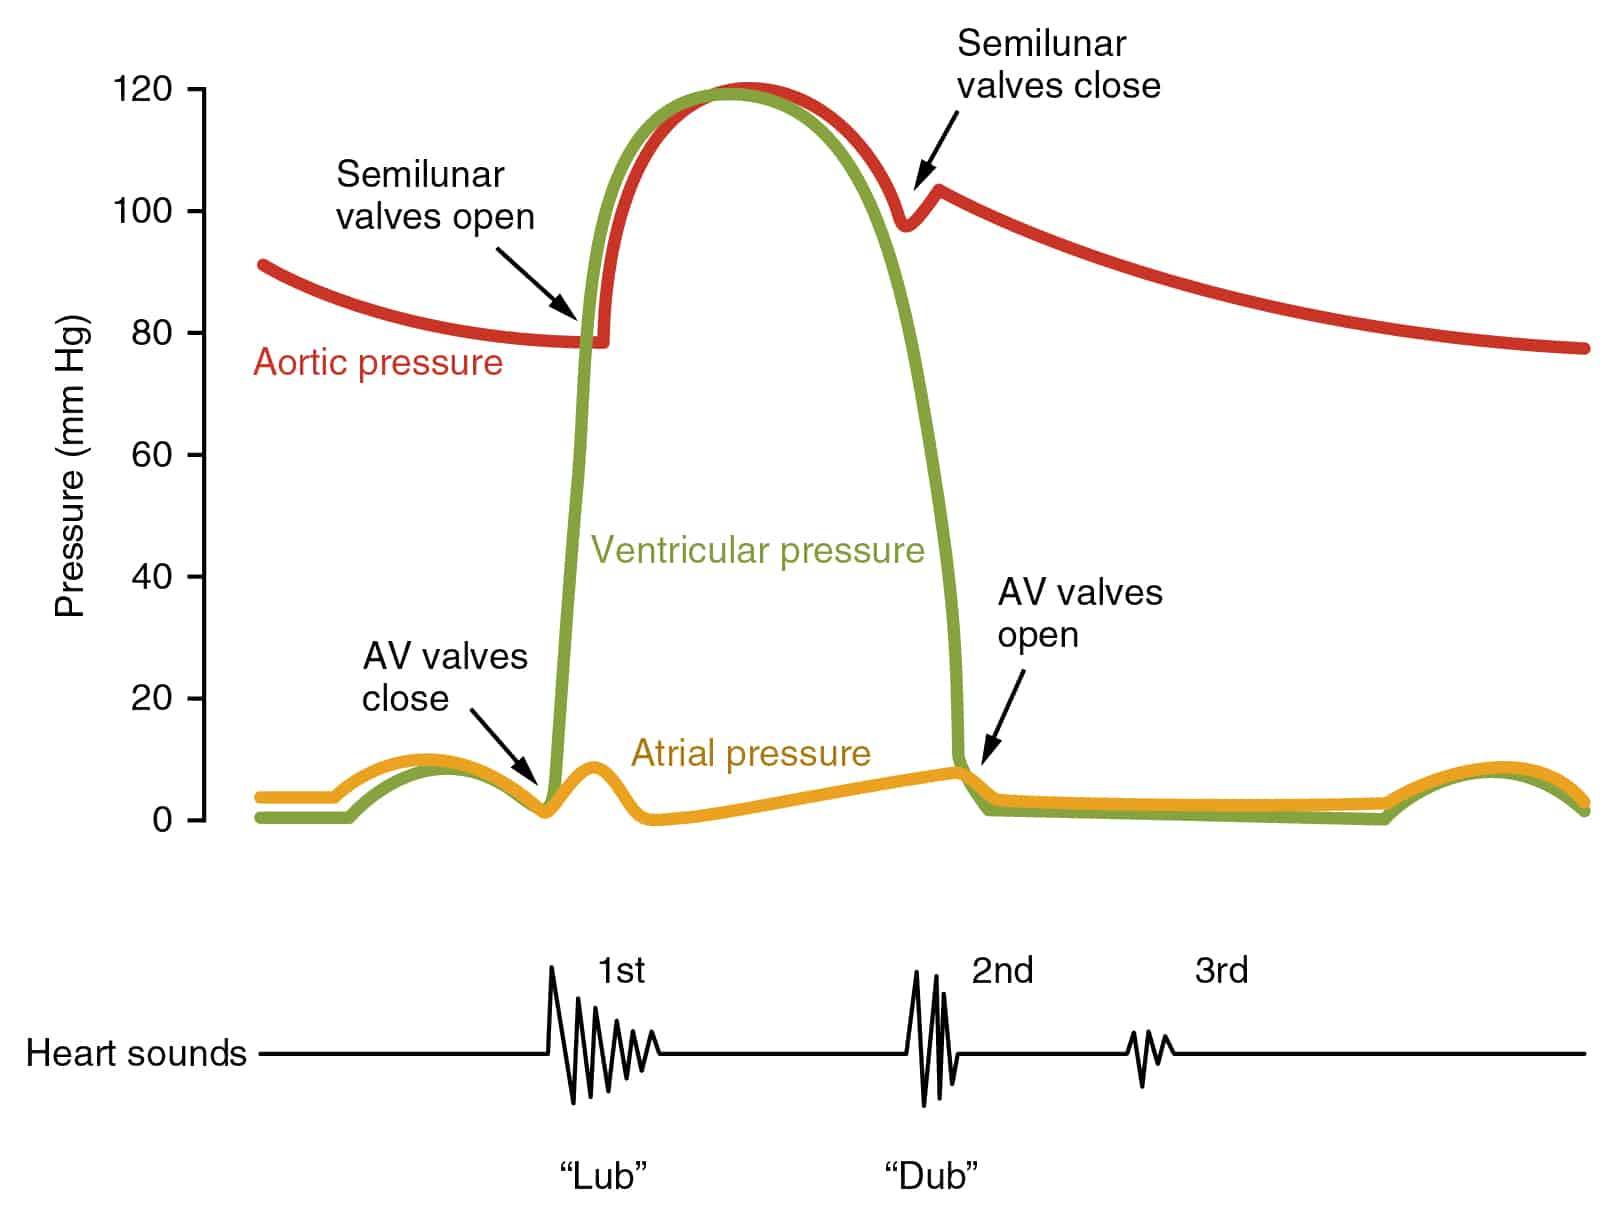
\includegraphics[width=\textwidth]{images/pressure-profile.jpg}
}
\note{
    \textbf{Tahmid}
}

\frame{
    \frametitle{Control: objectives}

    \begin{block}{Goal}
        Track and approach a target pressure profile in real time.
    \end{block}

    \begin{alertblock}{Constraints}
        \begin{itemize}
            \item Must not exceed maximum safe pressure --- vessel bursting is irreversible
            \item Must account for system non-linearities: syringe mechanics, valve dynamics
        \end{itemize}
    \end{alertblock}
}
\note{
    \textbf{India}

    \begin{itemize}
        \item Not just steady state pressure, track continuously varying waveform in real time
        \item Burst constraint is hard, overshooting once ruptures vessel --- be conservative
        \item Non-linearities --- may get dead zones from switching, tubing compliance stores energy, fluid inertia lags (does not fit linear systems)
        \item Strategy --- sample rapidly so each step stays near linear
    \end{itemize}
}


\frame{
    \frametitle{Control: solution}

    \begin{block}{Linear systems negative feedback loop}
        \begin{itemize}
            \item Filter raw pressure sensor output
            \item PID controller maps pressure error $\to$ motor speed
            \item High sampling frequency (${\sim}\SI{50}{\hertz}$) minimises non-linearity effects by keeping each control step within a near-linear operating region
            \item Control both the DC mean pressure component and the AC pulsatile waveform
        \end{itemize}
    \end{block}

    \begin{alertblock}{Key challenge: modelling the plant}
        Specifically the relationship between motor speed and output pressure.
    \end{alertblock}
}
\note{
    \footnotesize
    \textbf{India}

    \begin{itemize}
        \item Negative feedback loop --- filter $\rightarrow$ PID $\rightarrow$ motor speed command
        \item Filter first to remove high-frequency noise before computing error
        \item PID terms:
              \begin{itemize}
                  \item P term: immediate response to current error
                  \item I term: corrects persistent mean pressure offset
                  \item D term: damping to prevent overshoot
              \end{itemize}
        \item Controlling DC and AC simultaneously --- mean pressure set by average motor speed, pulsatile shape by modulating speed cyclically using pinch valves downstream
        \item DC and AC interact --- changing mean flow rate affects valve operating point
        \item Biggest unknown: plant model --- all of the unknowns sit between motor and sensor --- cannot set PID gains until this has been well characterised
    \end{itemize}
}

\frame{
    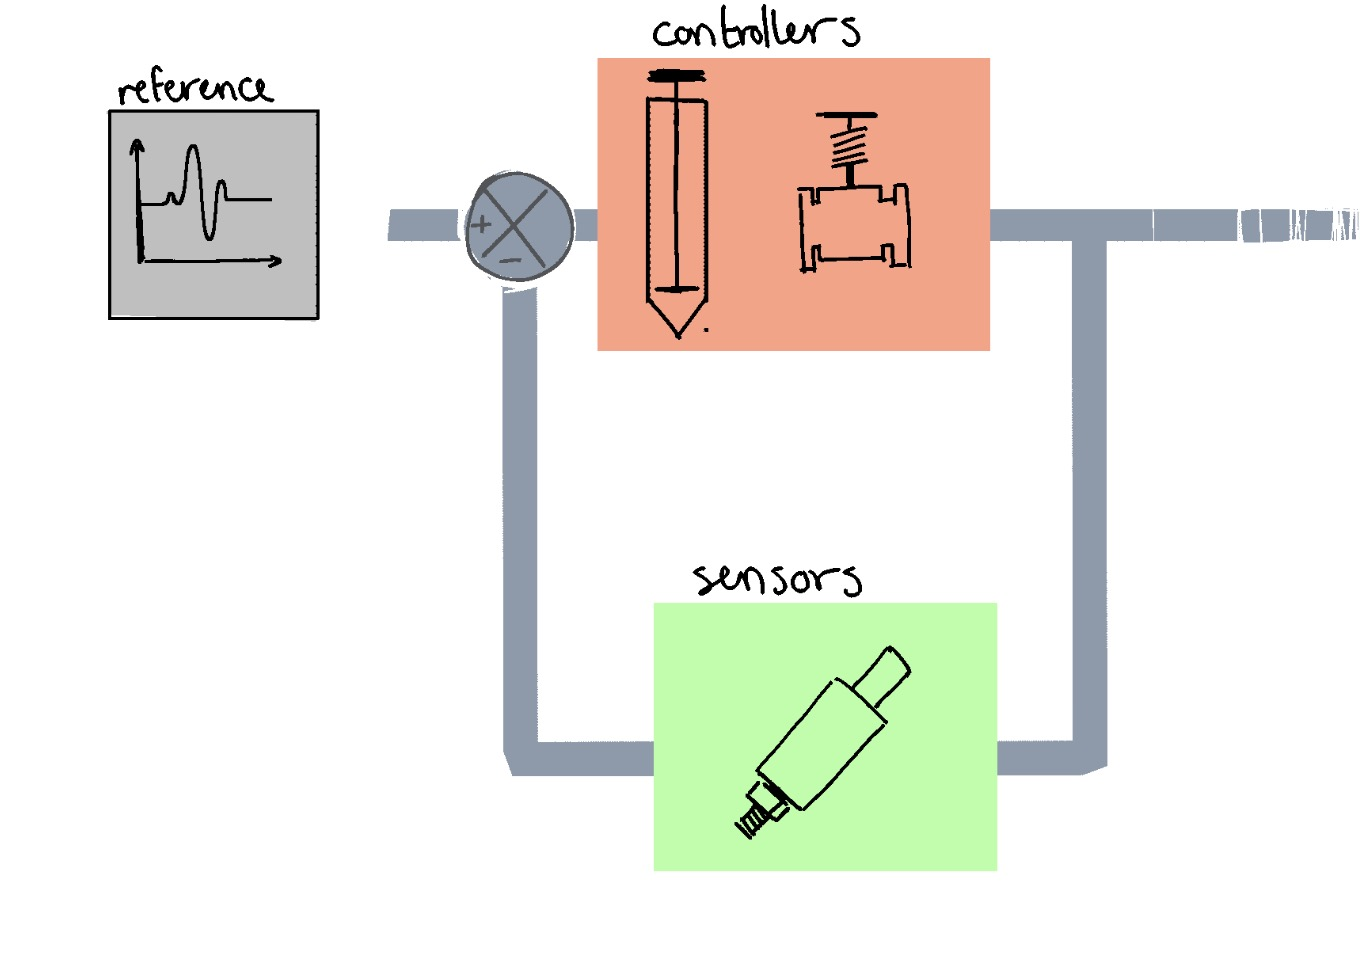
\includegraphics[width=\textwidth]{images/control.jpg}
}
\note{
    \textbf{India}

    \begin{itemize}
        \item Reference waveform comes in from software --- generated as Tahmid explained
        \item Compute error between reference and measured
        \item Controllers block are the actual actuators (plant)
        \item Sensors --- read pressure and close the loop
        \item Everything between motor and measurement point is in loop --- why plant model is really important
    \end{itemize}
}


\frame{
    \frametitle{Control: extensions}

    \begin{block}{Compliance modelling}
    \end{block}

    \begin{block}{Burst pressure modelling}
        \begin{itemize}
            \item Combine deformation gradients with pressure data to predict failure point
            \item Enables safe, more controlled burst pressure testing
        \end{itemize}
    \end{block}
}

\note{
    \textbf{India}

    \begin{itemize}
        \item Compliance modelling --- log pressure and vessel deformation continuously to build compliance curve across operating range
        \item Burst pressure modelling --- ramp to failure can be hard to control
        \item Use deformation gradients as indicator --- vessel shows characteristic change in response as they approach failure
        \item Track inflection point in real time --- safer and reproducible burst pressure measurement
    \end{itemize}
}


\frame{
    \frametitle{Next steps: initial prototype + testing}

    \small
    \begin{columns}[t, onlytextwidth]
        \column{0.48\textwidth}
        \begin{block}{Mechanical}
            \begin{itemize}
                \item Build syringe $\to$ valves $\to$ reservoir $\to$ syringe fluid circuit
                \item Build motor/syringe housing
                \item Connect pressure sensors to tubing
            \end{itemize}
        \end{block}

        \begin{block}{Electrical}
            \begin{itemize}
                \item Learn microcontroller software
            \end{itemize}
        \end{block}


        \column{0.48\textwidth}

        \begin{block}{Control}
            \begin{itemize}
                \item Build and test control system on simulated pressure waveforms
                \item Characterise controller lag and amplitude response in real time
            \end{itemize}
        \end{block}

        \begin{block}{Software}
            \begin{itemize}
                \item Choose a tech stack
                \item Begin basic modelling features and plan UIs
            \end{itemize}
        \end{block}
    \end{columns}
}
\note{
    \begin{itemize}
        \item Mechanical --- Lucy \& Luca
        \item Control --- India
              \begin{itemize}
                  \item Run PID against simulated waveforms to develop gains before even touching vessel
                  \item Open loop tests once mechanical circuit is ready to characterise plant model
              \end{itemize}
        \item Electrical --- Lonnie
        \item Software --- Tahmid
    \end{itemize}
}


\frame{
    \frametitle{Fallback: if syringe system doesn't work as planned}

    \begin{columns}
        \begin{column}{0.6\textwidth}
            \begin{block}{Gravity-powered flow}
            \end{block}

            \begin{block}{Diaphragm for pressure pulses}
            \end{block}
        \end{column}

        \begin{column}{0.4\textwidth}
            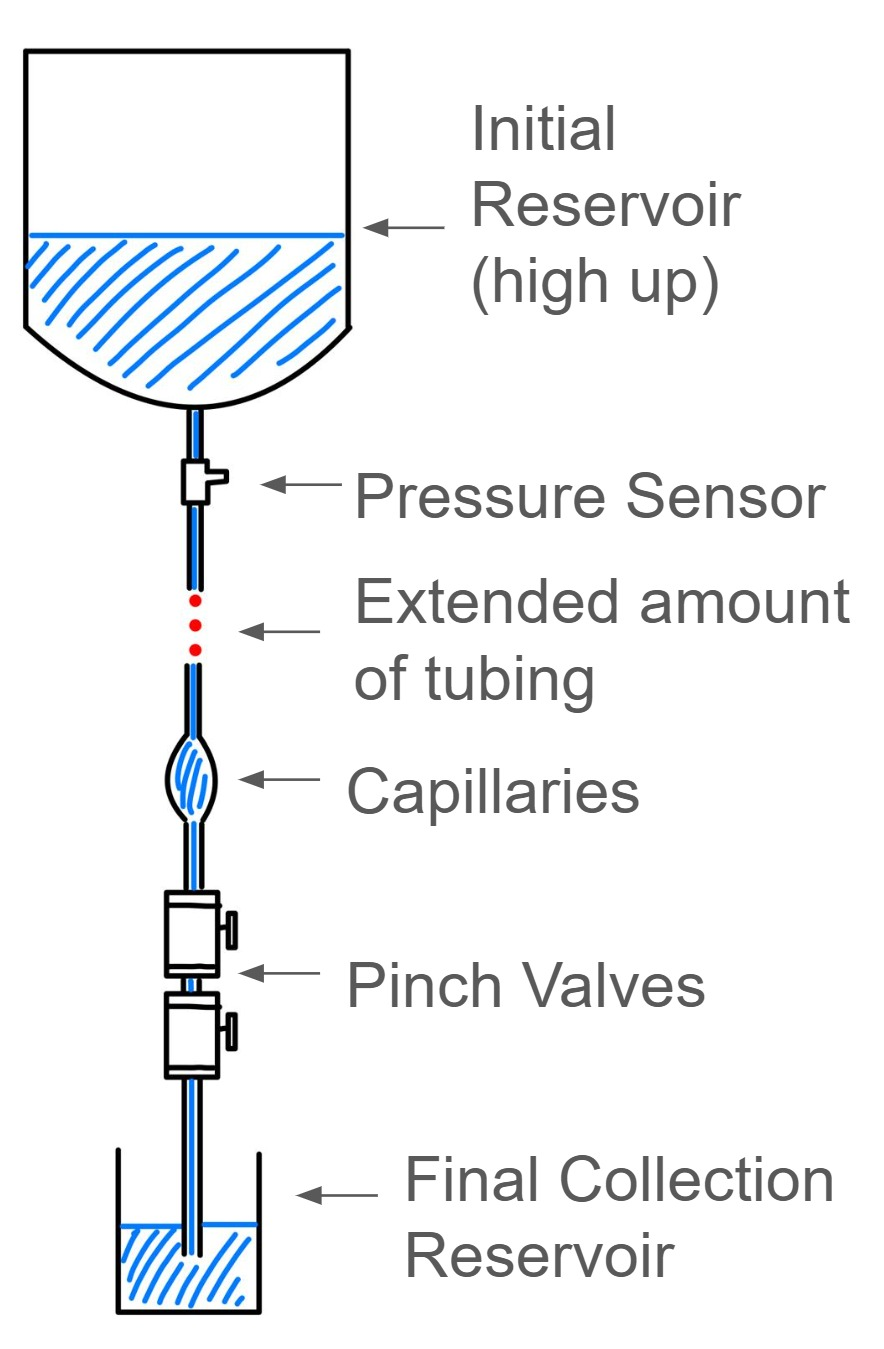
\includegraphics[width=\textwidth]{images/gravity.jpeg}
        \end{column}
    \end{columns}
}
\note{Lonnie}


\frame{
    \frametitle{References}
    \printbibliography[heading=none]
}

\frame{
    \frametitle{Questions?}


    \footnotesize Presentation source can be found at \underline{\href{www.github.com/tahmidazam/gm1-pump}{www.github.com/tahmidazam/gm1-pump}}.
}

\end{document}